\documentclass[a4paper,oneside,12pt]{article}
\usepackage{graphics,multicol}
\usepackage[latin1]{inputenc}
\usepackage[a4paper,margin=2cm,lmargin=2cm,headheight=1pt]{geometry}
\usepackage{fancyhdr}
\usepackage{amsmath,amssymb,amsfonts,amsthm, mathrsfs}
\usepackage{mathtools,bbm}
\usepackage{IEEEtrantools}
\usepackage[]{algorithm2e}
\usepackage{tikz,pgfplots,tkz-graph}
\usepackage{ifthen,calc}
\usepackage{listings,hyperref,float}
\usepackage{epsfig,epstopdf,graphicx}
\usepackage{enumerate}

\pgfplotsset{compat=newest}
\usetikzlibrary{positioning,matrix}
\interdisplaylinepenalty=2500

% Page settings
% \setlength{\oddsidemargin}{0 in}
% \setlength{\evensidemargin}{0 in}
% \setlength{\topmargin}{-0.6 in}
% \setlength{\textwidth}{6.5 in}
% \setlength{\textheight}{8.5 in}
% \setlength{\headsep}{0.75 in}
% \setlength{\parindent}{0 in}
% \setlength{\parskip}{0.1 in}

% Markov symbol X -o- Y
\newcommand{\markov}{\mathrel{\multimap}\joinrel\mathrel{-}\joinrel\mathrel{\mkern-6mu}\joinrel\mathrel{-}}
% Independent & not independent symbol X _||_ Y
\newcommand{\indep}{\mathrel{\bot}\joinrel\mathrel{\mkern-5mu}\joinrel\mathrel{\bot}}
\newcommand{\dep}{\centernot\indep}
% i.i.d.
\newcommand{\iid}{\stackrel{\mathrm{i.i.d.}}{\sim}}
% Integration d
\newcommand{\dd}{\mathop{}\!\mathrm{d}}

% Single braces
\newcommand{\agbrs}[1]{\left\langle #1 \right\rangle}	% angle braces,  	< x >
\newcommand{\rdbrs}[1]{\left( #1 \right)}				% round braces,  	( x )
\newcommand{\sqbrs}[1]{\left\lbrack #1 \right\rbrack}	% square braces, 	[ x ]
\newcommand{\clbrs}[1]{\left\lbrace #1 \right\rbrace}	% curly braces, 	{ x }

% Delimited braces
\newcommand{\agbrsv}[2]{\left\lange #1 \,\middle|\, #2 \right\rangle}	% angle braces with delimiter |,  	< x | y >, inner product
\newcommand{\rdbrsv}[2]{\left( #1 \,\middle|\, #2 \right)}				% round braces with delimiter |,  	( x | y ), conditional probability
\newcommand{\sqbrsv}[2]{\left\lbrack #1 \,\middle|\, #2 \right\rbrack}	% square braces with delimiter |,  	[ x | y ], conditional expectation
\newcommand{\clbrsv}[2]{\left\lbrace #1 \,\middle|\, #2 \right\rbrace}	% curly braces with delimiter |,  	{ x | y }, set

% Short for underline and overline
\newcommand{\udl}[1]{\underline{#1}}
\newcommand{\ovl}[1]{\overline{#1}}

% Derivative and partial derivation
\newcommand{\fracd}[2]{ \frac{\mathrm{d} #1}{\mathrm{d} #2} }
\newcommand{\fracp}[2]{ \frac{\partial #1}{\partial #2} }

% Absolute value, norm, ceil, floor, and evaluation
\newcommand{\abs}[1]{\left| #1 \right|}		% Absolute value, 	| x |
\newcommand{\norm}[1]{\left\| #1 \right\|}	% Norm, 			|| x ||
\DeclarePairedDelimiter\ceil{\lceil}{\rceil}
\DeclarePairedDelimiter\floor{\lfloor}{\rfloor}
\newcommand{\eval}[1]{\left. #1 \right|}	% Evaluation, 		f(x) |_{x=x0}

% Definition equal sign
\newcommand{\defeq}{\vcentcolon=}   % :=
\newcommand{\eqdef}{=\vcentcolon}   % =:
\newcommand{\texteq}[1]{\stackrel{#1}{=\joinrel=\joinrel=}}   % use for change of variable

% Inverse hyperbolic functions
\DeclareMathOperator\arcsinh{arcsinh}
\DeclareMathOperator\arccosh{arccosh}
\DeclareMathOperator\arctanh{arctanh}
\DeclareMathOperator\atanh{atanh}
\DeclareMathOperator\sech{sech}

% argmax and argmin
\newcommand\limit[1]{\underset{#1}{\lim}\,}
\newcommand\argmax[1]{\mathrm{arg}\,\underset{#1}{\max}\,}
\newcommand\argmin[1]{\mathrm{arg}\,\underset{#1}{\min}\,}

% Matrices
\newcommand*\pmtx[1]{\begin{pmatrix}#1\end{pmatrix}}			% Matrix with round braces
\newcommand*\bmtx[1]{\begin{bmatrix}#1\end{bmatrix}}			% Matrix with square braces
\newcommand*\vmtx[1]{\begin{vmatrix}#1\end{vmatrix}}			% Determinant of matrix
\newcommand*\spmtx[1]{\rdbrs{\begin{smallmatrix}#1\end{smallmatrix}}}	% Small matrix with round braces
\newcommand*\sbmtx[1]{\sqbrs{\begin{smallmatrix}#1\end{smallmatrix}}}	% Small matrix with square braces
\newcommand*\svmtx[1]{\abs{\begin{smallmatrix}#1\end{smallmatrix}}}		% Determinant of small matrix
\newcommand{\sizecorr}[1]{\makebox[0cm]{\phantom{$\displaystyle #1$}}}	% Get size of an expression

% Theorem environments
\newtheorem{theorem}{Theorem}
\newtheorem{corollary}[theorem]{Corollary}
\newtheorem{lemma}[theorem]{Lemma}
\newtheorem{observation}[theorem]{Observation}
\newtheorem{proposition}[theorem]{Proposition}
\newtheorem{definition}[theorem]{Definition}
\newtheorem{claim}[theorem]{Claim}
\newtheorem{fact}[theorem]{Fact}
\newtheorem{assumption}[theorem]{Assumption}

\newtheorem*{theorem*}{Theorem}
\newtheorem*{corollary*}{Corollary}
\newtheorem*{lemma*}{Lemma}
\newtheorem*{proposition*}{Proposition}
\newtheorem*{definition*}{Definition}
\newtheorem*{example*}{Example}
\newtheorem*{remark*}{Remark}
\newtheorem*{problem*}{Problem}

% Solution environment
\newenvironment{solution}{\begin{proof}[Solution]}{\end{proof}}

% Short for boldsymbol
\newcommand{\bs}[1]{\boldsymbol{#1}}

% Other frequent used operators
\def\Var{\mathsf{Var}}
\def\Cov{\mathsf{Cov}}
\def\coeff{\mathsf{coeff}}
\def\Tr{\mathsf{Tr}}
\def\rank{\mathsf{rank}}
\def\diag{\mathsf{diag}}
\def\mse{\mathsf{mse}}
\def\mmse{\mathsf{mmse}}

\def\ee{\mathbbm{e}}
\def\ii{\mathbbm{i}}
\def\EE{\mathsf{E}}
\def\FF{\mathsf{F}}
\def\SS{\mathsf{S}}
\def\UU{\mathsf{U}}
\def\xx{\mathsf{x}}
\def\pprime{{\prime\prime}}

\newcommand{\KL}[2]{D\left( #1 \,\middle|\middle|\, #2 \right)}%                   ( | )

\makeatletter
\newcommand\ztag[1]{%
\def\@currentlabel{#1}%
\gdef\tmp{%
\addtocounter{equation}{-1}%
\def\theequation{#1}}%
\aftergroup\aftergroup\aftergroup\aftergroup\aftergroup\aftergroup
\aftergroup\aftergroup\aftergroup\aftergroup\aftergroup\aftergroup
\aftergroup\aftergroup\aftergroup\aftergroup\aftergroup\aftergroup
\aftergroup\aftergroup\aftergroup\aftergroup\aftergroup\aftergroup
\aftergroup\aftergroup\aftergroup\aftergroup\aftergroup\aftergroup
\aftergroup
\tmp\IEEEyesnumber}


\pagestyle{empty}
\begin{document}

\noindent

\begin{tabular}{lcr}
  Duke University & & Math 690-40 \\  
  Homework four & \hspace{6.3cm} & F. Krzakala and L. Zdeborov\'a\\ \hline
\end{tabular}

\begin{center}
  {\Large {\bf Matrix Factorization and Applications}}
\end{center}

\subsection*{Reminder}
%%
We have studied in class the following problem: given a vector $ \mathbf{x}^* $, where each component $ x_i^* $ is taken from $ P_X(x) $, one is given a noisy symmetric $ N \times N $ matrix $ \mathbf{Y} $ such that
\begin{equation}
    Y_{ij} = \sqrt{ \frac{\lambda}{N} } x_i^* x_j^* + \omega_{ij} \label{def}
\end{equation}
where $ \lambda $ is the signal to noise ratio, and where $ \omega_{ij} = \omega_{ji} $ is a noise taken from a Gaussian distribution $ \mathcal{N}(0,1) $. 
We have seen that the free entropy reads $ \Phi(\lambda) = \min_m \Phi_{\mathrm{RS}}(m; \lambda) $ where $ m \ge 0 $ and
\begin{equation*}
    \Phi_{\mathrm{RS}}(m; \lambda)
    = -\frac{\lambda m^2}{4} + \int P_X(x^*) \dd x^* ~ \int \frac{ \ee^{-z^2/2} }{ \sqrt{2\pi} } \dd z ~ \log \clbrs{ \int P_X(x) \dd x ~ \exp \rdbrs{ -\frac{\lambda m}{2} x^2 + \lambda m x^* x + \sqrt{\lambda m} z x } }
\end{equation*}
and the maximizer $ m^*(\lambda) $ is the magnetization $ m = \mathbb{E}_{\mathbf{x}^*, \bs{\omega}} \sqbrs{ \agbrs{ \frac{1}{N} \sum_i x_i^* x_i }_{\mathbf{x}^*, \bs{\omega}} } $. 
We remind that the Minimum Mean Square Error is given by 
\begin{equation*}
    \mathsf{MMSE}(\lambda) = \mathbb{E}_{x^*} \sqbrs{ \rdbrs{ x^* }^2 } - m^*(\lambda)
\end{equation*}

\subsection*{A. Application to a binary estimation problem}

\begin{enumerate}[(a)]
\item   Assume now that each $ x_i^* = \pm 1 $ with equal probabilities, and show that one can then drastically simplify the expression of the free entropy such that only one integral (over $ z $) remains.
\item   Compute (numerically) the MMSE as function of $ \lambda $ and show that there is a phase transition at $ \lambda = 1 $.
\end{enumerate}
\begin{solution} $\,$ 
\begin{enumerate}[(a)]
\item 
        Since now we have $ P_X(x) = \frac{1}{2} \sqbrs{ \delta(x-1) + \delta(x+1) } $, we can simplify as
        \begin{IEEEeqnarray*}{rCl}
            \IEEEeqnarraymulticol{3}{l}{
                \int P_X(x) \dd x ~ \exp \rdbrs{ -\frac{\lambda m}{2} x^2 + \lambda m x^* x + \sqrt{\lambda m} z x }    
            }\nonumber\\* \quad
            &=& \frac{1}{2} \sqbrs{ \exp \rdbrs{ -\frac{\lambda m}{2} + \lambda m x^* + \sqrt{\lambda m} z } + \exp \rdbrs{ -\frac{\lambda m}{2} - \lambda m x^* - \sqrt{\lambda m} z } } \\
            &=& \ee^{-\frac{\lambda m}{2}} \cosh \rdbrs{ \lambda m x^* + \sqrt{\lambda m} z } \\
            \Phi_{\mathrm{RS}}(m; \lambda)
            &=& -\frac{\lambda m^2}{4} + \int P_X(x^*) \dd x^* ~ \int \frac{ \ee^{-z^2/2} }{ \sqrt{2\pi} } \dd z ~ \log \sqbrs{ \ee^{-\frac{\lambda m}{2}} \cosh \rdbrs{ \lambda m x^* + \sqrt{\lambda m} z } } \\
            &=& -\frac{\lambda m^2}{4} + \int P_X(x^*) \dd x^* ~ \int \frac{ \ee^{-z^2/2} }{ \sqrt{2\pi} } \dd z ~ \sqbrs{ -\frac{\lambda m}{2} + \log \clbrs{ \cosh \rdbrs{ \lambda m x^* + \sqrt{\lambda m} z } } } \\
            &=& -\frac{\lambda m^2}{4} + \frac{1}{2} \int \frac{ \ee^{-z^2/2} }{ \sqrt{2\pi} } \dd z ~ \sqbrs{ -\frac{\lambda m}{2} + \log \clbrs{ \cosh \rdbrs{ \lambda m + \sqrt{\lambda m} z } } } \\
            && + \frac{1}{2} \int \frac{ \ee^{-z^2/2} }{ \sqrt{2\pi} } \dd z ~ \sqbrs{ -\frac{\lambda m}{2} + \log \clbrs{ \cosh \rdbrs{ -\lambda m + \sqrt{\lambda m} z } } } \\
            &=& -\frac{\lambda m^2}{4} - \frac{\lambda m}{2} + \frac{1}{2} \mathbb{E}_z \sqbrs{ \log \clbrs{ \frac{1}{2} \rdbrs{ \cosh(2 \lambda m) + \cosh( 2z \sqrt{\lambda m} ) } } }
        \end{IEEEeqnarray*}
\item 
        The $ \Phi_{\mathrm{RS}}(m;\lambda) $ function is plotted over range $ m \in [0, 1] $ and $ m \in [0, 0.1] $ with $ \lambda \in \clbrs{ 0.5, 0.75, 1, 1.05, 1.1 } $.
        \begin{figure}[H]
            \centering
            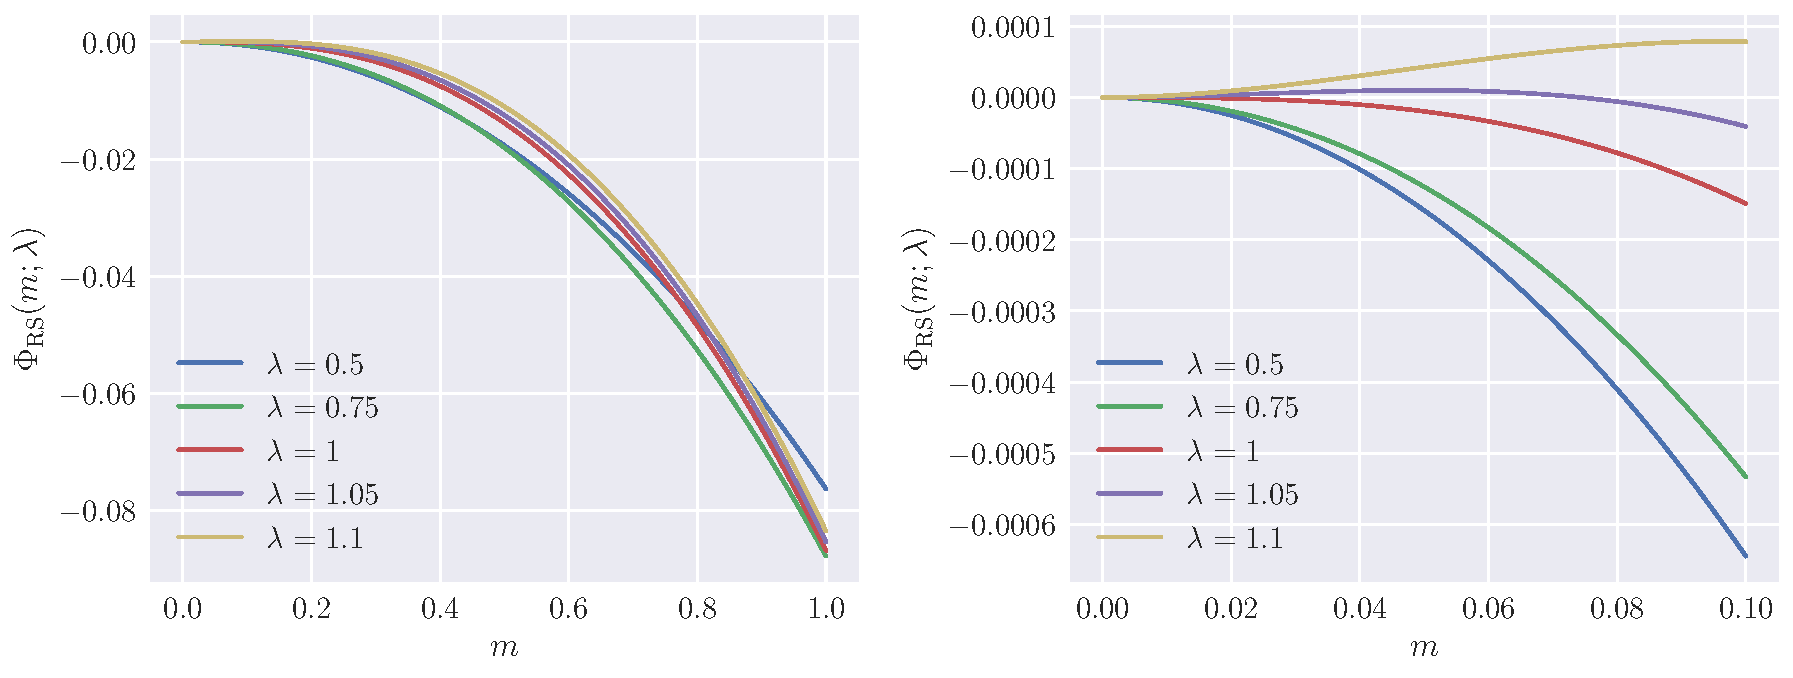
\includegraphics[width=\textwidth]{hw4/hw4_1(b)1.pdf}
        \end{figure}
        To compute $ m^* $ as a function of $ \lambda $, notice that it is the maximizer of $ \Phi_{\mathrm{RS}}(m; \lambda) $, so we have the consistency equation by solving
        \begin{IEEEeqnarray*}{rCl}
            0 
            &=& \fracp{}{m} \Phi_{\mathrm{RS}}(m; \lambda) 
            = -\frac{\lambda m}{2} - \frac{\lambda}{2} + \frac{1}{2} \mathbb{E}_z \sqbrs{ \frac{ 2 \lambda \sinh \rdbrs{ 2 \lambda m } + \frac{\lambda z}{\sqrt{\lambda m}} \sinh \rdbrs{ 2z \sqrt{\lambda m} } }{ \cosh(2 \lambda m) + \cosh( 2z \sqrt{\lambda m} ) } } \\
            \Rightarrow \quad
            m &=& \mathbb{E}_z \sqbrs{ \frac{ 2 \sinh \rdbrs{ 2 \lambda m } + \frac{z}{\sqrt{\lambda m}} \sinh \rdbrs{ 2z \sqrt{\lambda m} } }{ \cosh(2 \lambda m) + \cosh( 2z \sqrt{\lambda m} ) } } - 1
        \end{IEEEeqnarray*}
        Finally, for the MMSE, it is straightforward to see
        \begin{equation*}
            \mathbb{E}_{x^*} \sqbrs{ \rdbrs{ x^* }^2 } = 1
            \quad \Rightarrow \quad
            \mathsf{MMSE}(\lambda) = \mathbb{E}_{x^*} \sqbrs{ \rdbrs{ x^* }^2 } - m^*(\lambda) = 1 - m^*(\lambda)
        \end{equation*}
        \begin{figure}[H]
            \centering
            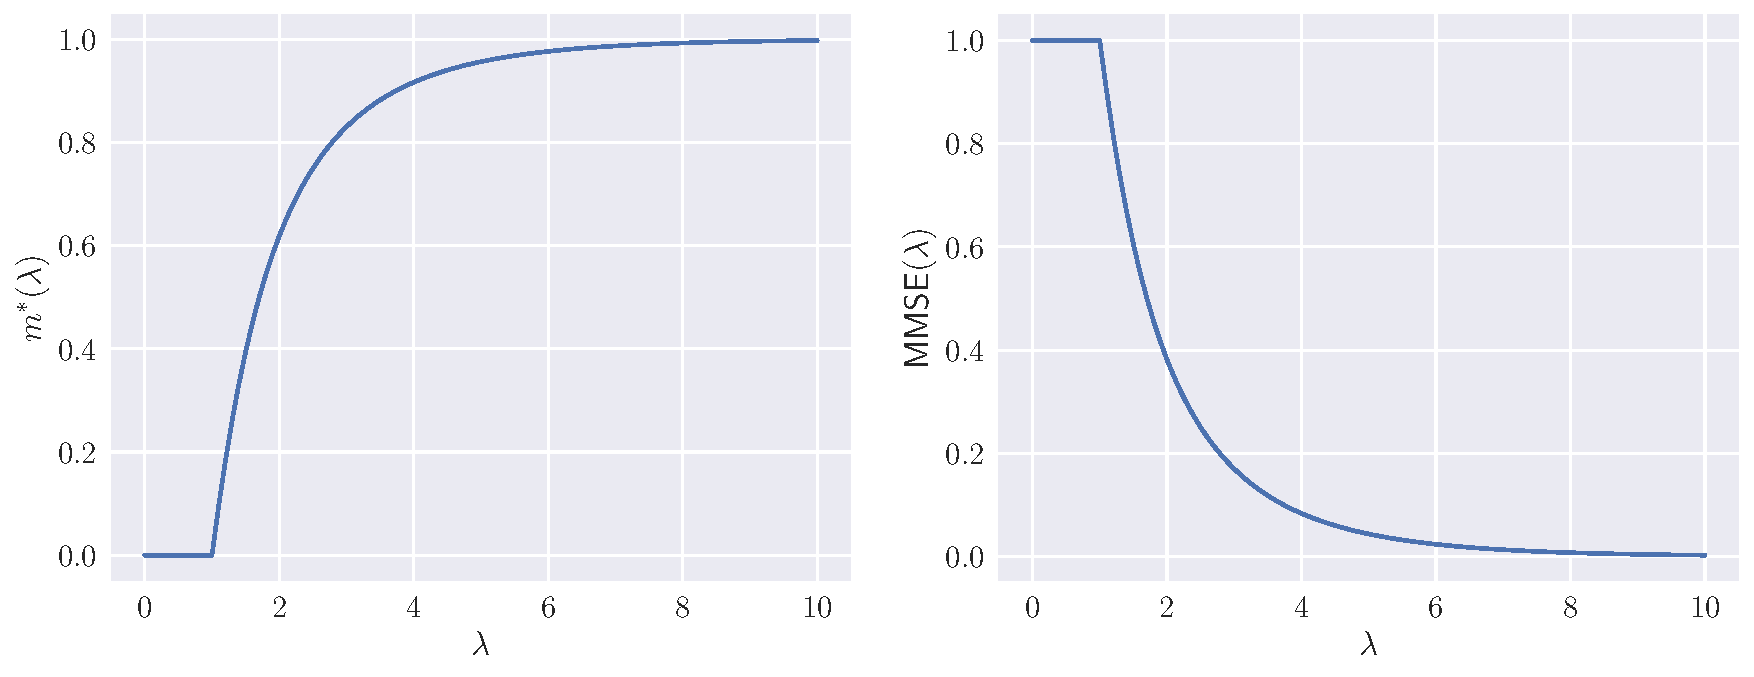
\includegraphics[width=\textwidth]{hw4/hw4_1(b)2.pdf}
        \end{figure}
        Again, it is easy to see that $ m^*(\lambda) $ leaves $ 0 $ continuously when $ \lambda \ge 1 $, indicating a second-order phase transition.
\end{enumerate}
\end{solution}


\subsection*{B. Comparison to a spectral algorithm}

Let us compare the theoretical performance with the one of a particular algorithm: spectral clustering. 
In spectral clustering, we estimate the unknown $ \mathbf{x}^* $ as follow: 
(i) we compute the leading (largest) eigenvalue of $ \mathbf{Y} $ and 
(ii) we estimate $ \hat{x}_i = \mathsf{sign}(v_i) $, where $ \mathbf{v} $ is the eigenvector corresponding the largest eigenvalue.

For several values of $ N $ compute the mean square error of the spectral method as a function of $ \lambda $ (note that since we cannot know if the solution is $ \hat{\mathbf{x}} $ or $ -\hat{\mathbf{x}} $ we should try both):
\begin{equation*}
    \mathsf{MSE}_{\mathrm{spectral}}(N, \lambda)
    = \min \rdbrs{ \frac{1}{N} \sum_i \rdbrs{ x_i^* - \hat{x}_i }^2, \frac{1}{N} \sum_i \rdbrs{ x_i^* + \hat{x}_i }^2 }
\end{equation*}
and compare $ \mathsf{MSE}_{\mathrm{spectral}}(N, \lambda) $ with the theoretical predictions at $ N \to \infty $.
How would you rate the performance of the spectral algorithm?
\begin{solution} $\,$ 
For the simulation, I choose $ N \in \clbrs{ 100, 200, 500, 1000 } $, over $ \lambda \in [0, 10] $, each data point is averaged over $ 100 $ trials.
\begin{figure}[H]
    \centering
    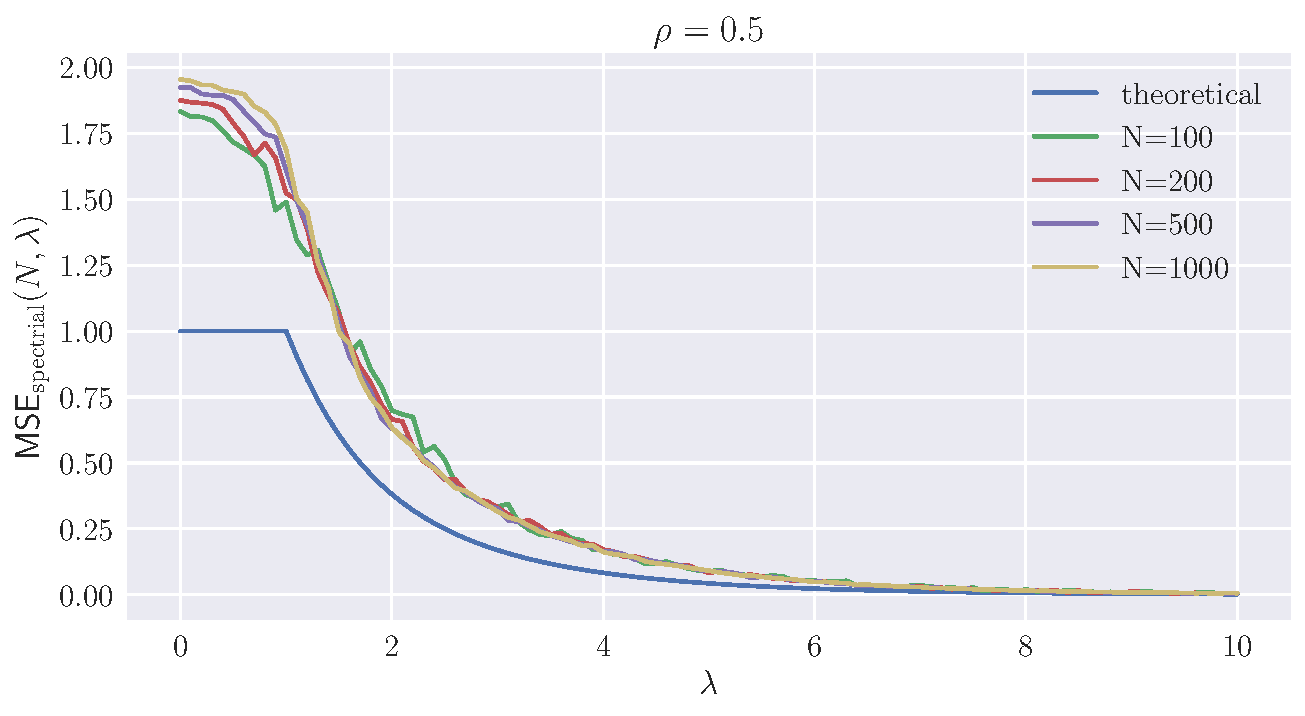
\includegraphics[width=400pt]{hw4/hw4_2.pdf}
\end{figure}
It can be seen that the MSE of spectral algorithm is about twice larger than the theoretical curve.
This is because the MMSE estimation uses posterior mean, which is a `soft' decision, to give a explicit clustering partition one needs to make hard decision over those posterior mean.
Spectral algorithm, on the other hand, gives hard decision directly, where the event $ \hat{x}_i = 0 $ occurs with probability zero.

Actually, to give a fair comparison, one needs to implement AMP algorithm to compute `soft' $ \hat{\mathbf{x}} $, make hard decision based on it and then compute the MSE of AMP algorithm.
\end{solution}

\subsection*{C. A sparse variation} 
Repeat the previous analysis when $ x_i^* = \sqrt{ (1-\rho) / \rho } $ with probability $ \rho = 0.075 $ and $ -\sqrt{ \rho / (1-\rho) } $ with probability $ 1-\rho = 0.925 $. 
Adapt the clustering algorithm in this case, and compare its performance with the theoretical curve.  
How would you rate the performance of the spectral algorithm this time?
\begin{solution} $\,$ 
Using similar tricks as the first problem, we obtain
\begin{IEEEeqnarray*}{rCl}
    \IEEEeqnarraymulticol{3}{l}{
        \int P_X(x) \dd x ~ \exp \rdbrs{ -\frac{\lambda m}{2} x^2 + \lambda m x^* x + \sqrt{\lambda m} z x }    
    }\nonumber\\* \quad
    &=& \rho \exp \rdbrs{ -\frac{\lambda m}{2} \frac{1-\rho}{\rho} + \lambda m \sqrt{ \frac{1-\rho}{\rho} } x^* + \sqrt{\lambda m} \sqrt{ \frac{1-\rho}{\rho} } z } \\
    && + (1-\rho) \exp \rdbrs{ -\frac{\lambda m}{2} \frac{\rho}{1-\rho} - \lambda m \sqrt{ \frac{\rho}{1-\rho} } x^* - \sqrt{\lambda m} \sqrt{ \frac{\rho}{1-\rho} } z }
\end{IEEEeqnarray*}
Unfortunately, there is no easy way to simplify this expression to a more compact form.

Plugging in the above results yields
\begin{IEEEeqnarray*}{rCl}
    \Phi_{\mathrm{RS}}(m; \lambda)
    &=& -\frac{\lambda m^2}{4} \\
    && + \rho \, \mathbb{E}_z \Biggl[
    \log \Biggl\{
    \rho \exp \rdbrs{ \frac{\lambda m}{2} \frac{1-\rho}{\rho} + \sqrt{\lambda m} \sqrt{ \frac{1-\rho}{\rho} } z } \\
    && \qquad \qquad \quad + (1-\rho) \exp \rdbrs{ -\frac{\lambda m}{2} \rdbrs{ \frac{\rho}{1-\rho} + 2 } - \sqrt{\lambda m} \sqrt{ \frac{\rho}{1-\rho} } z } 
    \Biggr\} \Biggr]  \\
    && + (1-\rho) \, \mathbb{E}_z \Biggl[ \log \Biggl\{
    \rho \exp \rdbrs{ -\frac{\lambda m}{2} \rdbrs{ \frac{1-\rho}{\rho} + 2 } + \sqrt{\lambda m} \sqrt{ \frac{1-\rho}{\rho} } z } \\
    && \qquad \qquad \quad + (1-\rho) \exp \rdbrs{ \frac{\lambda m}{2} \frac{\rho}{1-\rho} - \sqrt{\lambda m} \sqrt{ \frac{\rho}{1-\rho} } z } 
    \Biggr\} \Biggr]
\end{IEEEeqnarray*}
The $ \Phi_{\mathrm{RS}}(m;\lambda) $ function is plotted over range $ m \in [0, 1] $ and $ m \in [0, 0.1] $ with $ \lambda \in \clbrs{ 0.5, 0.75, 1, 1.05, 1.1 } $.
\begin{figure}[H]
    \centering
    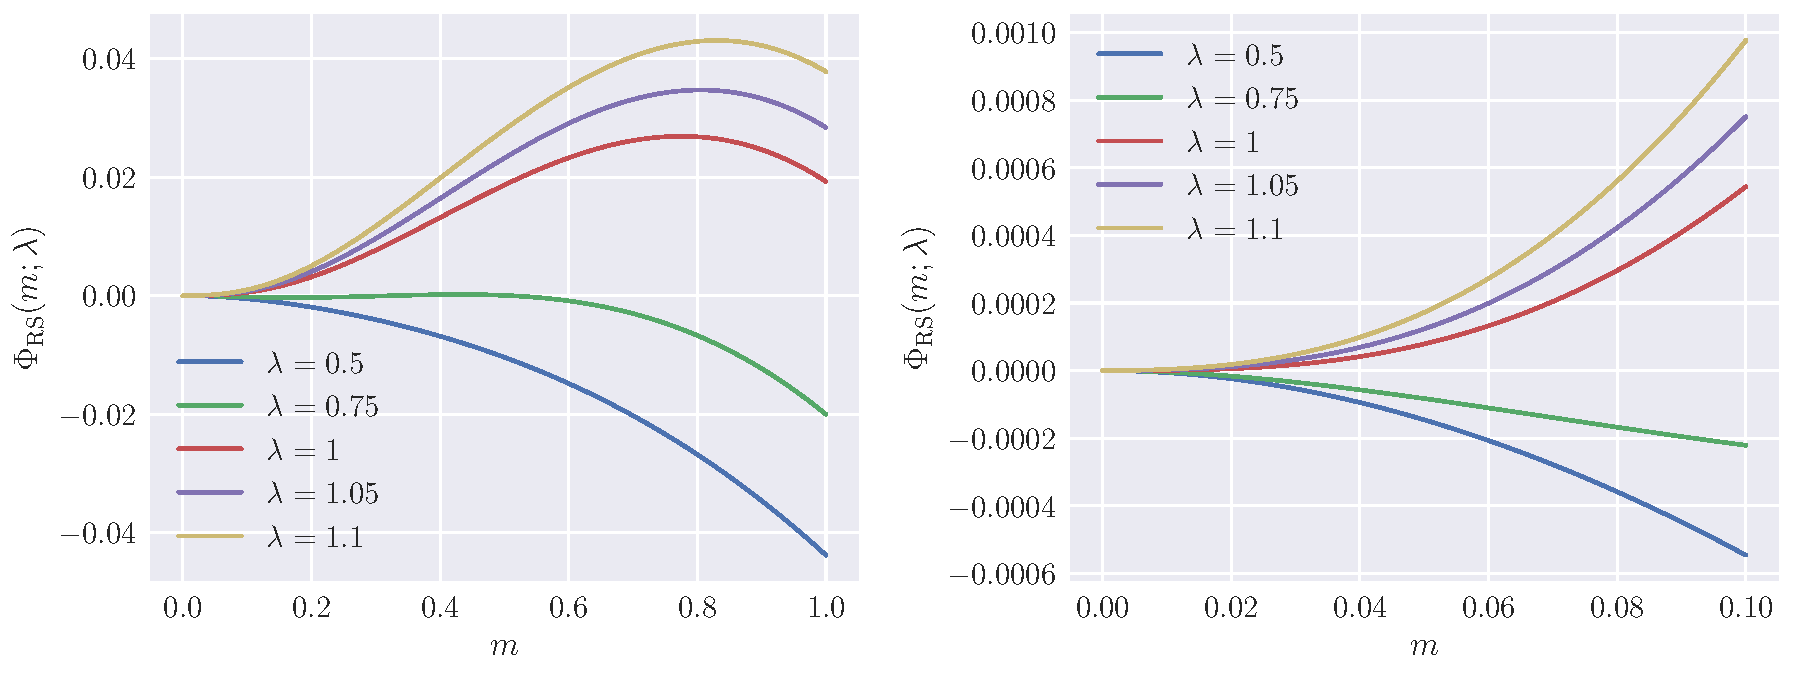
\includegraphics[width=\textwidth]{hw4/hw4_3(a)1.pdf}
\end{figure}
Similarly, to compute $ m^*(\lambda) $, we need to find the self-consistency equation
\begin{IEEEeqnarray*}{rCl}
    0 &=& \fracp{}{m} \Phi_{\mathrm{RS}}(m; \lambda)
    = -\frac{\lambda m}{2} + \mathbb{E}_z \sqbrs{ \rho T_1 + (1-\rho) T_2 } \\
    T_1
    &=& \frac{ \rdbrs{ \frac{\lambda (1-\rho)}{2} + \frac{z}{2} \sqrt{ \frac{\lambda \rho (1-\rho)}{m} } } \ee^{ \frac{\lambda m}{2} \frac{1-\rho}{\rho} + \sqrt{\lambda m} \sqrt{ \frac{1-\rho}{\rho} } z } + \rdbrs{ -\frac{\lambda (2-\rho)}{2} - \frac{z}{2} \sqrt{ \frac{\lambda \rho (1-\rho)}{m} } } \ee^{ -\frac{\lambda m}{2} \rdbrs{ \frac{\rho}{1-\rho} + 2 } - \sqrt{\lambda m} \sqrt{ \frac{\rho}{1-\rho} } z }  }{ \rho \ee^{ \frac{\lambda m}{2} \frac{1-\rho}{\rho} + \sqrt{\lambda m} \sqrt{ \frac{1-\rho}{\rho} } z } + (1-\rho) \ee^{ -\frac{\lambda m}{2} \rdbrs{ \frac{\rho}{1-\rho} + 2 } - \sqrt{\lambda m} \sqrt{ \frac{\rho}{1-\rho} } z } } \\
    T_2
    &=& \frac{ \rdbrs{ -\frac{\lambda (1+\rho)}{2} + \frac{z}{2} \sqrt{ \frac{\lambda \rho (1-\rho)}{m} } }\ee^{ -\frac{\lambda m}{2} \rdbrs{ \frac{1-\rho}{\rho} + 2 } + \sqrt{\lambda m} \sqrt{ \frac{1-\rho}{\rho} } z } + \rdbrs{ \frac{\lambda \rho}{2} - \frac{z}{2} \sqrt{ \frac{\lambda \rho (1-\rho)}{m} } } \ee^{ \frac{\lambda m}{2} \frac{\rho}{1-\rho} - \sqrt{\lambda m} \sqrt{ \frac{\rho}{1-\rho} } z }  }{ \rho \ee^{ -\frac{\lambda m}{2} \rdbrs{ \frac{1-\rho}{\rho} + 2 } + \sqrt{\lambda m} \sqrt{ \frac{1-\rho}{\rho} } z } + (1-\rho) \ee^{ \frac{\lambda m}{2} \frac{\rho}{1-\rho} - \sqrt{\lambda m} \sqrt{ \frac{\rho}{1-\rho} } z }  }
\end{IEEEeqnarray*}
So the self-consistency equation is
\begin{equation*}
    m = \frac{2}{\lambda} \mathbb{E}_z \sqbrs{ \rho T_1 + (1-\rho) T_2 }
\end{equation*}
Solving for $ m^*(\lambda) $ numerically, finally we get to the MMSE, it is straightforward to see
\begin{equation*}
    \mathbb{E}_{x^*} \sqbrs{ \rdbrs{ x^* }^2 } = \rho \frac{1-\rho}{\rho} + (1-\rho) \frac{\rho}{1-\rho} = 1
    \quad \Rightarrow \quad
    \mathsf{MMSE}(\lambda) = \mathbb{E}_{x^*} \sqbrs{ \rdbrs{ x^* }^2 } - m^*(\lambda) = 1 - m^*(\lambda)
\end{equation*}
\begin{figure}[H]
    \centering
    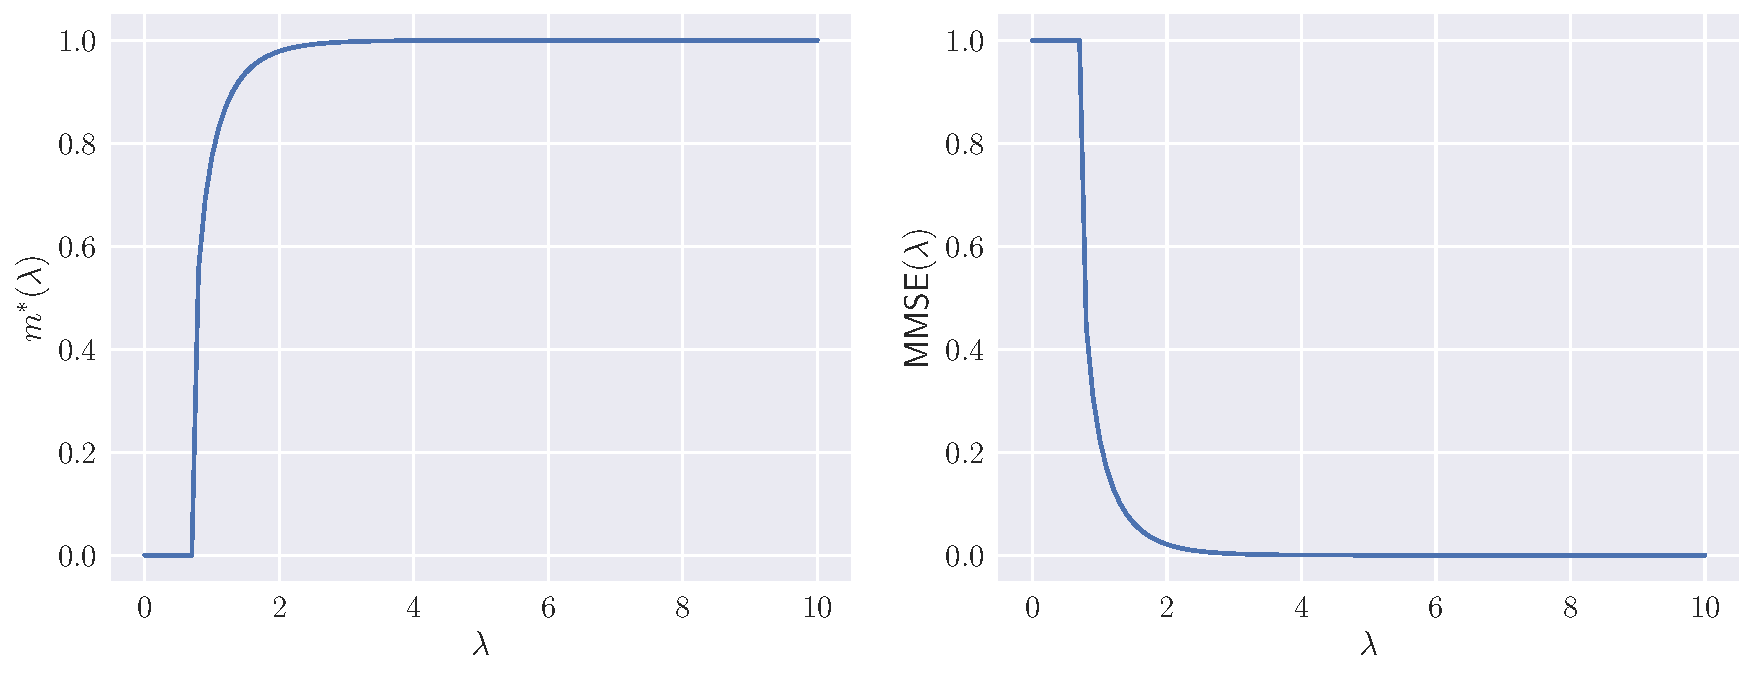
\includegraphics[width=\textwidth]{hw4/hw4_3(a)2.pdf}
\end{figure}
The phase transition occurs at $ \lambda \approx 0.746 $.

To make the spectral algorithm works for the unbalanced case, we need to slightly change the algorithm as follows:
\begin{enumerate}[(1)]
\item   Find the eigenvector $ \mathbf{v} $ associated to the largest eigenvalue in the sense of absolute value
\item   Find the set of indices of first $ N \rho $ smallest elements in $ \mathbf{v} $, call it $ \mathcal{I}^+ $, similarly do this for $ -\mathbf{v} $ and get $ \mathcal{I}^- $.
\item   Compute $ \hat{\mathbf{x}}^+ $ and $ \hat{\mathbf{x}}^- $ by
        \begin{equation*}
            \hat{x}_i^+ = 
            \begin{cases}
                \sqrt{ \frac{1-\rho}{\rho} }, &\text{ if } i \in \mathcal{I}^+\\
                -\sqrt{ \frac{\rho}{1-\rho} }, &\text{ if } i \notin \mathcal{I}^+\\
            \end{cases}, \qquad
            \hat{x}_i^- = 
            \begin{cases}
                \sqrt{ \frac{1-\rho}{\rho} }, &\text{ if } i \in \mathcal{I}^-\\
                -\sqrt{ \frac{\rho}{1-\rho} }, &\text{ if } i \notin \mathcal{I}^-\\
            \end{cases}, \qquad
        \end{equation*}
\item   Choose the one with smaller error, i.e.
        \begin{equation*}
            \mathsf{MSE}_{\mathrm{spectral}}(N, \lambda)
            = \min \rdbrs{ \frac{1}{N} \sum_i \rdbrs{ x_i^* - \hat{x}_i^+ }^2, \frac{1}{N} \sum_i \rdbrs{ x_i^* - \hat{x}_i^- }^2 }
        \end{equation*}
\end{enumerate}


At the end, let's compare the performance between spectral algorithm and the theoretical curve:
\begin{figure}[H]
    \centering
    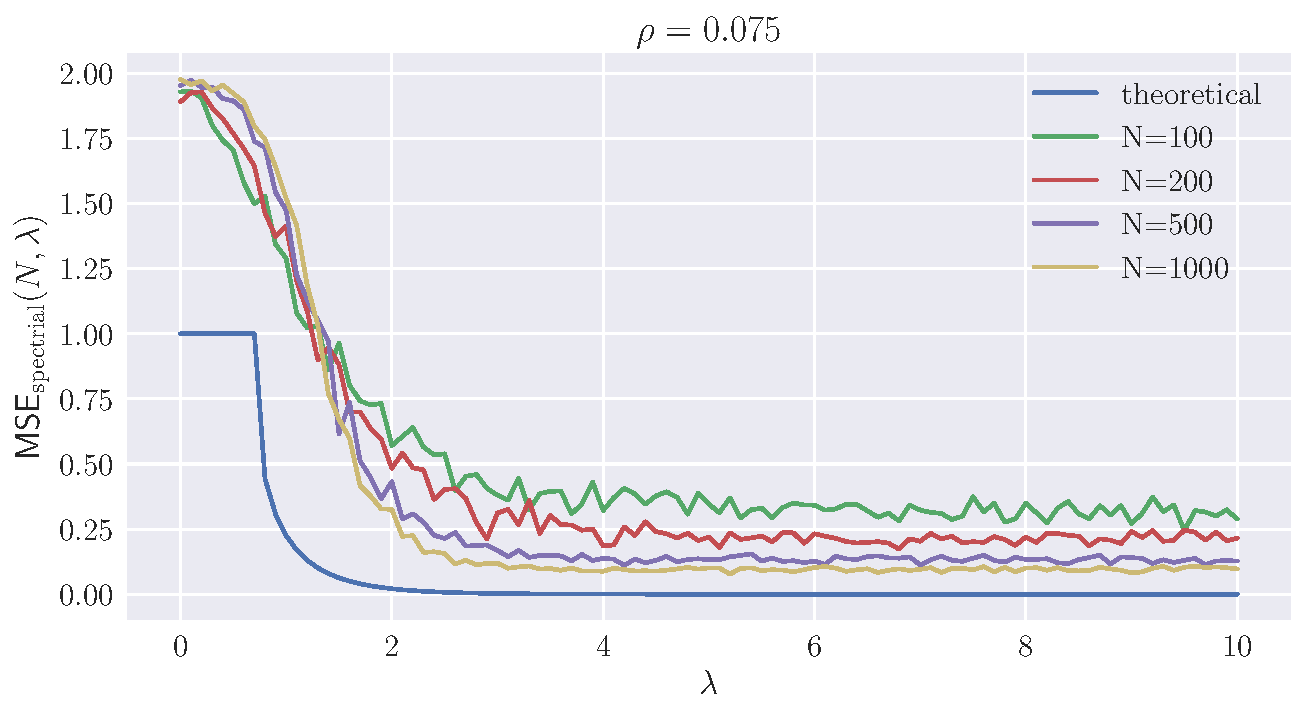
\includegraphics[width=400pt]{hw4/hw4_3.pdf}
\end{figure}
In contrast, the theoretical MMSE curve is much lower, which means spectral algorithm performs far away from the theoretical optimal bound.
\end{solution}


\subsection*{D. Community Detection variation} 
This time picture the values $ x_i^* = 1 $ as being in one group, and $ x_i^* = -1 $ as being in another group. 
Instead on observing $ Y_{ij} $ as in eq.~(\ref{def}) we have that 
\begin{IEEEeqnarray*}{rCl}
    P \rdbrs{ Y_{ij} = 1 } &=& p_{\mathrm{out}} + \frac{\mu}{\sqrt{N}} x_i^* x_j^* \\
    P \rdbrs{ Y_{ij} = 0 } &=& 1 - p_{\mathrm{out}} - \frac{\mu}{\sqrt{N}} x_i^* x_j^* \\
\end{IEEEeqnarray*}
\begin{enumerate}[(a)]
\item   Using the universality principle we have seen in class, show that this is a particular case of the Stochastic Block Model as defined in the very first lecture. 
\item   Use the universality theorem that maps a generic output channel into the Gaussian one using Fisher information. Give the expression between $ \lambda $, and $ p_{\mathrm{out}} $ and $ \mu $ in this mapping. 
\end{enumerate}
\begin{solution} $\,$ 
\begin{enumerate}[(a)]
\item 
        We have nodes in two groups with $ x_i^* \in \clbrs{ \pm 1 } $ with $ x_i \sim P_X(x) = (1-\rho) \, \delta(x+1) + \rho \, \delta(x-1) $.
        Also, we can view $ Y_{ij} $ as the indicator of whether there is an edge connecting node $ i $ and node $ j $
        Therefore, the problem is converted into
        \begin{equation*}
            \begin{cases}
                P \rdbrsv{ (ij) \in E }{ x_i^*, x_j^* } = P(Y_{ij} = 1) = p_{x_i^*, x_j^*} \\
                P \rdbrsv{ (ij) \notin E }{ x_i^*, x_j^* } = P(Y_{ij} = 0) = 1 - p_{x_i^*, x_j^*}
            \end{cases}
            \quad \Rightarrow \quad
            p_{x_i^*, x_j^*} = p_{\mathrm{out}} + \frac{\mu}{\sqrt{N}} x_i^* x_j^*
        \end{equation*}
        Now, we have
        \begin{itemize}
        \item   number of groups: $ 2 $
        \item   the faction of each community: $ p_{-1} = 1 - \rho $, $ p_{+1} = \rho $
        \item   a symmetric $ 2 \times 2 $ matrix of edge probabilities
                \begin{equation*}
                    \bmtx{ p_{\mathrm{out}} + \frac{\mu}{\sqrt{N}} & p_{\mathrm{out}} - \frac{\mu}{\sqrt{N}} \\ p_{\mathrm{out}} - \frac{\mu}{\sqrt{N}} & p_{\mathrm{out}} + \frac{\mu}{\sqrt{N}} }
                \end{equation*}
        \end{itemize}
        which is sufficient to define an SBM.
\item   Mapping this problem into a symmetric vector-spin glass model:
        \begin{IEEEeqnarray*}{rCl}
            P \rdbrsv{ \mathbf{x} }{ \mathbf{Y} }
            &=& \frac{1}{Z(\mathbf{Y})} \prod_i P_X(x_i) \prod_{i \le j} \ee^{g \rdbrs{ Y_{ij}, \frac{x_i x_j}{\sqrt{N}} } }
        \end{IEEEeqnarray*}
        where
        \begin{equation*}
            g \rdbrs{ y, z } 
            = \log \rdbrs{ \rdbrs{ p_{\mathrm{out}} + \mu z }^y \rdbrs{ 1 - p_{\mathrm{out}} - \mu z }^{1-y} } 
            = \log \rdbrs{ 1 - p_{\mathrm{out}} - \mu z } + y \log \rdbrs{ \frac{ p_{\mathrm{out}} + \mu z }{ 1 - p_{\mathrm{out}} - \mu z } }
        \end{equation*}
        Define
        \begin{IEEEeqnarray*}{rCl}
            S(Y_{ij})
            &\equiv& \eval{ \fracp{g(Y_{ij}, z)}{z} }_{z=0}
            = \frac{ (Y_{ij}-p_{\mathrm{out}}) \mu }{ p_{\mathrm{out}} (1-p_{\mathrm{out}}) }
            % R(Y_{ij})
            % &\equiv& \rdbrs{ \eval{ \fracp{g(Y_{ij}, z)}{z} }_{z=0} }^2 + \eval{ \frac{\partial^2 g(Y_{ij}, z)}{\partial z^2} }_{z = 0}
            % = -\frac{ Y_{ij} (1-Y_{ij}) \mu^2 }{ p_{\mathrm{out}}^2 \rdbrs{ 1-p_{\mathrm{out}} }^2 } \\
        \end{IEEEeqnarray*}
        Hence, evaluating at $ Y_{ij} \in \clbrs{ 0, 1 } $ gives
        \begin{equation*}
            S(Y_{ij} = 1) = \frac{\mu}{p_{\mathrm{out}}}, \quad
            S(Y_{ij} = 0) = -\frac{\mu}{1-p_{\mathrm{out}}}
            % R(Y_{ij} = 1) = R(Y_{ij} = 0) = 0
        \end{equation*}
        The inverse Fisher information is defined as
        \begin{IEEEeqnarray*}{rCl}
            \mathbb{E}_{Y \mid z = 0} \sqbrs{ \rdbrs{ \eval{ \fracp{}{z} \log \rdbrs{ P \rdbrsv{ Y }{ z } } }_{z=0} }^2 }
            &=& \mathbb{E}_{Y \mid z = 0 } \sqbrs{ \rdbrs{ \eval{ \fracp{g(Y, z)}{z} }_{z=0} }^2 } 
            = \mathbb{E}_{Y \mid z = 0 } \sqbrs{ S^2(Y) } \\
            &=& (1-p_{\mathrm{out}})  S^2(0) + p_{\mathrm{out}} S^2(1) 
            = \frac{ \mu^2 }{ p_{\mathrm{out}} \rdbrs{ 1 - p_{\mathrm{out}} } }
        \end{IEEEeqnarray*}
        On the other hand, consider the channel in the class, we have
        \begin{equation*}
            Y_{ij} = \sqrt{\lambda} \frac{x_i^* x_j^*}{\sqrt{N}} + \xi_{ij}, \qquad
            P \rdbrsv{ y }{ z } = \frac{1}{\sqrt{2\pi}} \exp \rdbrs{ -\frac{1}{2} \rdbrs{ y - \sqrt{\lambda} z }^2 }
        \end{equation*}
        In this case we have $ Y \mid z = 0 \sim \mathcal{N}(0,1) $ and the inverse Fisher information is
        \begin{IEEEeqnarray*}{rCl}
            \mathbb{E}_{Y \mid z = 0} \sqbrs{ \rdbrs{ \eval{ \fracp{}{z} \log \rdbrs{ P \rdbrsv{ Y }{ z } } }_{z=0} }^2 }
            &=& \int \frac{ \ee^{-\frac{y^2}{2}} }{\sqrt{2\pi}} \dd y ~ \sqbrs{ \eval{ \sqrt{\lambda} \rdbrs{ y - \sqrt{\lambda} z } }_{z=0} }^2 \\
            &=& \lambda \int y^2 \frac{ \ee^{-\frac{y^2}{2}} }{\sqrt{2\pi}} \dd y = \lambda
        \end{IEEEeqnarray*}
        Finally, the relationship between $ \lambda $, $ p_{\mathrm{out}} $ and $ \mu $ is
        \begin{equation*}
            \lambda = \frac{ \mu^2 }{ p_{\mathrm{out}} \rdbrs{ 1 - p_{\mathrm{out}} } }
        \end{equation*}
\end{enumerate}
\end{solution}

\subsection*{E. State Evolution}
We have seen in class an algorithm called Approximate Message Passing. 
The interesting things about it is that we can predict exactly its dynamics by analyzing the so-called "state evolution" equation that states that
%
\begin{equation*}
    m^{(t+1)} = \mathbb{E}_{x^*, z} \sqbrs{ \rdbrs{ f \rdbrs{ \lambda m^{(t)}, \lambda m^{(t)} x^* + \sqrt{ \lambda m^{(t)} } z } }^2 }
\end{equation*}
where
\begin{equation*}
    f(A, B) = \frac{ \int \dd x ~ x P_X^0(x) \ee^{ -\frac{A}{2} x^2 + B x } }{ \int \dd x ~ P_X^0(x) \ee^{ -\frac{A}{2} x^2 + B x } }
\end{equation*}
Show that the state evolution equation is a fixed point of the replica free entropy.

Given this, which one of the problems discussed so far should be solved by AMP (in the sense that AMP reached the Bayes-Optimal MSE)? 
Would AMP outperforms spectral methods in question B and C ? 
If yes, in which sense.
\begin{solution} $\,$ 
\begin{enumerate}[(a)]
\item 
We start with the replica free entropy at Bayes-optimal case where $ P_X \equiv P_X^0 $:
        \begin{IEEEeqnarray*}{rCl}
            \Phi_{\mathrm{RS}}(m; \lambda) 
            &=& -\frac{\lambda m^2}{4} + \mathbb{E}_{x^*, z} \sqbrs{ \log \rdbrs{ \int P_X^0(x) \dd x ~ \ee^{ -\frac{\lambda m}{2} x^2 + \rdbrs{ \lambda m x^* + \sqrt{\lambda m} z } x } } }
        \end{IEEEeqnarray*}
        Therefore, taking partial derivative w.r.t. $ m $ and set it to zero gives
        \begin{IEEEeqnarray*}{rCl}
            0 &=& \fracp{}{m} \Phi_{\mathrm{RS}}(m; \lambda) \\
            &=& -\frac{\lambda m}{2} + \mathbb{E}_{x^*, z} \sqbrs{ \frac{ \fracp{}{m} \int P_X^0(x) \dd x ~ \ee^{ -\frac{\lambda m}{2} x^2 + \rdbrs{ \lambda m x^* + \sqrt{\lambda m} z } x } }{ \int P_X^0(x) \dd x ~ \ee^{ -\frac{\lambda m}{2} x^2 + \rdbrs{ \lambda m x^* + \sqrt{\lambda m} z } x } } } \\
            &=& -\frac{\lambda m}{2} + \mathbb{E}_{x^*, z} \sqbrs{ \frac{ \int P_X^0(x) \dd x ~ \ee^{ -\frac{\lambda m}{2} x^2 + \rdbrs{ \lambda m x^* + \sqrt{\lambda m} z } x } \sqbrs{ -\frac{\lambda}{2} x^2 + \lambda x^* x + \sqrt{\frac{\lambda}{m}} \frac{z}{2} x } }{ \int P_X^0(x) \dd x ~ \ee^{ -\frac{\lambda m}{2} x^2 + \rdbrs{ \lambda m x^* + \sqrt{\lambda m} z } x } } } \\
            &=& -\frac{\lambda m}{2} + \mathbb{E}_{x^*, z} \sqbrs{ \rdbrs{ \lambda x^* + \sqrt{ \frac{\lambda}{m} } z } f \rdbrs{ \lambda m, \lambda m x^* + \sqrt{\lambda m} z } - \frac{\lambda}{2} \frac{ \int \dd x ~ x^2 P_X^0(x) \ee^{ -\frac{A}{2} x^2 + B x } }{ \int \dd x ~ P_X^0(x) \ee^{ -\frac{A}{2} x^2 + B x } } } \\
            &\overset{(a)}{=}& -\frac{\lambda m}{2} + \mathbb{E}_{x^*, z} \Biggl[ \lambda x^* f \rdbrs{ \lambda m, \lambda m x^* + \sqrt{\lambda m} z } + \frac{1}{2} \sqrt{\frac{\lambda}{m}} \fracp{}{z} f \rdbrs{ \lambda m, \lambda m x^* + \sqrt{\lambda m} z } \\
            && \qquad \qquad \qquad \quad - \frac{\lambda}{2} \frac{ \int \dd x ~ x^2 P_X^0(x) \ee^{ -\frac{A}{2} x^2 + B x } }{ \int \dd x ~ P_X^0(x) \ee^{ -\frac{A}{2} x^2 + B x } } \Biggr] \\
            &\overset{(b)}{=}& -\frac{\lambda m}{2} + \mathbb{E}_{x^*, z} \Biggl[ \lambda x^* f \rdbrs{ \lambda m, \lambda m x^* + \sqrt{\lambda m} z } - \frac{\lambda}{2} \rdbrs{ f \rdbrs{ \lambda m, \lambda m x^* + \sqrt{\lambda m} z } }^2 \Biggr] \\
            &\overset{(c)}{=}& -\frac{\lambda m}{2} + \frac{\lambda}{2} \mathbb{E}_{x^*, z} \Biggl[ \rdbrs{ f \rdbrs{ \lambda m, \lambda m x^* + \sqrt{\lambda m} z } }^2 \Biggr]
        \end{IEEEeqnarray*}
        where
        \begin{enumerate}[(a)]
        \item   Uses the Stein's lemma that $ z \sim \mathcal{N}(0,1) $, then
                \begin{equation*}
                    \mathbb{E}_z \sqbrs{ z f(z) } = \mathbb{E}_z \sqbrs{ \fracp{}{z} f(z) }
                \end{equation*}
        \item   Uses the fact that
                \begin{equation*}
                    \fracp{}{B} f(A, B)
                    = \frac{ \int \dd x ~ x P_X^0(x) \ee^{ -\frac{A}{2} x^2 + B x } }{ \int \dd x ~ P_X^0(x) \ee^{ -\frac{A}{2} x^2 + B x } } - \sqbrs{ f(A,B) }^2
                \end{equation*}
        \item   Uses the Nishimori identity that
                \begin{equation*}
                    \mathbb{E}_{x^*, z} \sqbrs{ x^* \agbrs{ x }_{x^*, z} }
                    = \mathbb{E}_{x^*, z} \sqbrs{ \agbrs{ x^* x }_{x^*, z} }
                    = \mathbb{E}_{x^*, z} \sqbrs{ \agbrs{ x^{(1)} x^{(2)} }_{x^*, z} }
                    = \mathbb{E}_{x^*, z} \sqbrs{ \agbrs{ x^{(1)} }_{x^*, z} \agbrs{ x^{(2)} }_{x^*, z} }
                \end{equation*}
                where $ x^{(1)}, x^{(2)} $ are two i.i.d. replicas distributed as $ P \rdbrsv{ x }{ \sqrt{\lambda} x^* + z } $ and the posterior mean is denoted as
                \begin{equation*}
                    \agbrs{ x }_{x^*, z} 
                    = \frac{ \int \dd x ~ x P_X^0(x) \ee^{ -\frac{\lambda m}{2} x^2 + \rdbrs{ \lambda m x^* + \sqrt{\lambda m} z } x } }{ \int \dd x ~ P_X^0(x) \ee^{ -\frac{\lambda m}{2} x^2 + \rdbrs{ \lambda m x^* + \sqrt{\lambda m} z } x } }
                    = f \rdbrs{ \lambda m, \lambda m x^* + \sqrt{\lambda m} z } 
                \end{equation*}
        \end{enumerate}
        Hence, finally we have the stationary condition
        \begin{equation*}
            m 
            = \mathbb{E}_{x^*, z} \sqbrs{ \rdbrs{ f \rdbrs{ \lambda m, \lambda m x^* + \sqrt{\lambda m} z } }^2 }
            = \mathbb{E}_{x^*, z} \sqbrs{ x^* f \rdbrs{ \lambda m, \lambda m x^* + \sqrt{\lambda m} z } },
        \end{equation*}
        which is exactly the state evolution equation.
\item 
        For Problem B and C, let's see what is their state evolution fixed point.
        First we have the prior
        \begin{IEEEeqnarray*}{rCl}
            P_X^0(x) 
            &=& \rho \delta \rdbrs{ x - \sqrt{ \frac{1-\rho}{\rho} } } + (1-\rho) \delta \rdbrs{ x + \sqrt{ \frac{\rho}{1-\rho} } } \\
            f(A,B)
            &=& \frac{ \sqrt{\rho (1-\rho)} \rdbrs{ \ee^{-\frac{A}{2} \frac{1-\rho}{\rho} + B \sqrt{\frac{1-\rho}{\rho}} } - \ee^{-\frac{A}{2} \frac{\rho}{1-\rho} - B \sqrt{\frac{\rho}{1-\rho}} } } }{ \rho \ee^{-\frac{A}{2} \frac{1-\rho}{\rho} + B \sqrt{\frac{1-\rho}{\rho}} } + (1-\rho) \ee^{-\frac{A}{2} \frac{\rho}{1-\rho} - B \sqrt{\frac{\rho}{1-\rho}} } } \\
            &=& \sqrt{\rho (1-\rho)} \frac{ 2\sinh \rdbrs{ h(A,B) } }{ \ee^{ -h(A,B) } + 2\rho \sinh \rdbrs{ h(A,B) } }
        \end{IEEEeqnarray*}
        where
        \begin{IEEEeqnarray*}{rCl}
            h(A,B)
            = -\frac{A}{4} \frac{1-2\rho}{\rho(1-\rho)} + \frac{B}{2} \rdbrs{ \sqrt{\frac{1-\rho}{\rho}} + \sqrt{\frac{\rho}{1-\rho}} }
            = -\frac{A}{4} \frac{1-2\rho}{\rho(1-\rho)} + \frac{B}{2 \sqrt{\rho(1-\rho)} }
        \end{IEEEeqnarray*}
        Therefore, for short we write $ A \triangleq \lambda m $ and $ B_\pm = \pm \lambda m \sqrt{\rdbrs{ \frac{1-\rho}{\rho} }^{\pm1}} + \sqrt{\lambda m} z $
        \begin{IEEEeqnarray*}{rCl}
            h(A,B_+)
            &=& h \rdbrs{ \lambda m, \lambda m \sqrt{\frac{1-\rho}{\rho}} + \sqrt{\lambda m} z }
            = \frac{1}{4} \sqbrs{ \frac{\lambda m}{\rho(1-\rho)} + 2z \sqrt{ \frac{\lambda m}{\rho(1-\rho)} } } \\
            h(A,B_-)
            &=& h \rdbrs{ \lambda m, -\lambda m \sqrt{\frac{\rho}{1-\rho}} + \sqrt{\lambda m} z }
            = \frac{1}{4} \sqbrs{ -\frac{\lambda m}{\rho(1-\rho)} + 2z \sqrt{ \frac{\lambda m}{\rho(1-\rho)} } }
        \end{IEEEeqnarray*}
        Notice that $ z \sim \mathcal{N}(0,1) $ is symmetric around $ 0 $, thus we have $ \mathbb{E}_z[g(z)] = \mathbb{E}_z[g(-z)] $ for any function $ g $
        \begin{IEEEeqnarray*}{rCl}
            \IEEEeqnarraymulticol{3}{l}{
                \mathbb{E}_z \sqbrs{ f(A, B_-) }
                = \mathbb{E}_z \sqbrs{ \sqrt{\rho (1-\rho)} \frac{ 2\sinh \rdbrs{ h(A,B_-) } }{ \ee^{ -h(A,B_-) } + 2\rho \ \sinh \rdbrs{ h(A,B_-) } } }
            }\nonumber\\* \quad
            &=& \mathbb{E}_z \sqbrs{ \frac{ \sqrt{\rho (1-\rho)} \cdot 2\sinh \rdbrs{ \frac{1}{4} \sqbrs{ -\frac{\lambda m}{\rho(1-\rho)} + 2z \sqrt{ \frac{\lambda m}{\rho(1-\rho)} } } } }{ \ee^{ -\frac{1}{4} \sqbrs{ -\frac{\lambda m}{\rho(1-\rho)} + 2z \sqrt{ \frac{\lambda m}{\rho(1-\rho)} } } } + 2\rho \ \sinh \rdbrs{ \frac{1}{4} \sqbrs{ -\frac{\lambda m}{\rho(1-\rho)} + 2z \sqrt{ \frac{\lambda m}{\rho(1-\rho)} } } } } } \\
            &=& \mathbb{E}_z \sqbrs{ \frac{ \sqrt{\rho (1-\rho)} \cdot 2\sinh \rdbrs{ \frac{1}{4} \sqbrs{ -\frac{\lambda m}{\rho(1-\rho)} - 2z \sqrt{ \frac{\lambda m}{\rho(1-\rho)} } } } }{ \ee^{ -\frac{1}{4} \sqbrs{ -\frac{\lambda m}{\rho(1-\rho)} - 2z \sqrt{ \frac{\lambda m}{\rho(1-\rho)} } } } + 2\rho \ \sinh \rdbrs{ \frac{1}{4} \sqbrs{ -\frac{\lambda m}{\rho(1-\rho)} - 2z \sqrt{ \frac{\lambda m}{\rho(1-\rho)} } } } } } \\
            &=& \mathbb{E}_z \sqbrs{ \sqrt{\rho (1-\rho)} \frac{ 2\sinh \rdbrs{ -h(A,B_+) } }{ \ee^{ h(A,B_+) } + 2\rho \ \sinh \rdbrs{ -h(A,B_+) } } } \\
            &=& -\mathbb{E}_z \sqbrs{ \sqrt{\rho (1-\rho)} \frac{ 2\sinh \rdbrs{ h(A,B_+) } }{ \ee^{ h(A,B_+) } - 2\rho \ \sinh \rdbrs{ h(A,B_+) } } }
        \end{IEEEeqnarray*}
        Hence, the state evolution equation can be rewritten as
        \begin{IEEEeqnarray*}{rCl}
            \IEEEeqnarraymulticol{3}{l}{
                \mathbb{E}_{x^*, z} \sqbrs{ x^* f \rdbrs{ \lambda m, \lambda m x^* + \sqrt{\lambda m} z } }
            }\nonumber\\* \quad
            &=& \rho \sqrt{ \frac{1-\rho}{\rho} } \mathbb{E}_z \sqbrs{ f(A, B_+) } - (1-\rho) \sqrt{ \frac{\rho}{1-\rho} } \mathbb{E}_z \sqbrs{ f(A,B_-) } \\
            &=& 2 \rho (1-\rho) \mathbb{E}_z \sqbrs{ \frac{ \sinh \rdbrs{ h(A,B_+) } }{ \ee^{ -h(A,B_+) } + 2\rho \sinh \rdbrs{ h(A,B_+) } } + \frac{ \sinh \rdbrs{ h(A,B_+) } }{ \ee^{ h(A,B_+) } - 2\rho \sinh \rdbrs{ h(A,B_+) } } } \\
            &=& 2 \rho (1-\rho) \mathbb{E}_z \sqbrs{ \frac{ 2 \sinh \rdbrs{ h(A, B_+) } \cosh \rdbrs{ h(A, B_+) } }{ 1 + 4 \rho (1-\rho) \sinh^2 \rdbrs{ h(A,B_+) } } } \\
            &=& 2 \rho (1-\rho) \mathbb{E}_z \sqbrs{ \frac{ \sinh \rdbrs{ 2h(A, B_+) } }{ 1 + 2 \rho (1-\rho) \sqbrs{ \cosh \rdbrs{ 2h(A,B_+) } - 1 } } } \\
            &=& \mathbb{E}_z \sqbrs{ \frac{ 2 \rho (1-\rho) \sinh \rdbrs{ \frac{\lambda m}{2\rho(1-\rho)} + z \sqrt{ \frac{\lambda m}{\rho(1-\rho)} } } }{ 1 + 2 \rho (1-\rho) \sqbrs{ \cosh \rdbrs{ \frac{\lambda m}{2\rho(1-\rho)} + z \sqrt{ \frac{\lambda m}{\rho(1-\rho)} } } - 1 } } }
        \end{IEEEeqnarray*}
        i.e. we can use the following state evolution iteration
        \begin{equation*}
            m^{(t+1)} = f^{\mathrm{SE}} \rdbrs{ \lambda m^{(t)} }, \quad
            f^{\mathrm{SE}}(x)
            = \int \frac{\ee^{-\frac{z^2}{2}}}{\sqrt{2\pi}} \dd z ~ \frac{ 2 \rho (1-\rho) \sinh \rdbrs{ \frac{x}{2\rho(1-\rho)} + z \sqrt{ \frac{x}{\rho(1-\rho)} } } }{ 1 + 2 \rho (1-\rho) \sqbrs{ \cosh \rdbrs{ \frac{x}{2\rho(1-\rho)} + z \sqrt{ \frac{x}{\rho(1-\rho)} } } - 1 } } 
        \end{equation*}
        AMP algorithm achieves the information theoretical MSE the problem is not in the hard phase.
        Hence, we can plot $ m^* $ versus $ \Delta = 1/\lambda $ to see if there exists a hard phase, i.e. if the interval $ [\Delta_{\mathrm{Alg}}, \Delta_{\mathrm{IT}}] $ exists.

        It can be seen that when $ \rho = 0.5 $, there is no hard phase so that AMP can achieve the Bayes-optimal MSE; when $ \rho = 0.075 $, the hard phase is $ \Delta \in [1, 1.3406] $, AMP converges to a strictly larger error than the Bayes-optimal MSE.
        \begin{figure}[H]
            \centering
            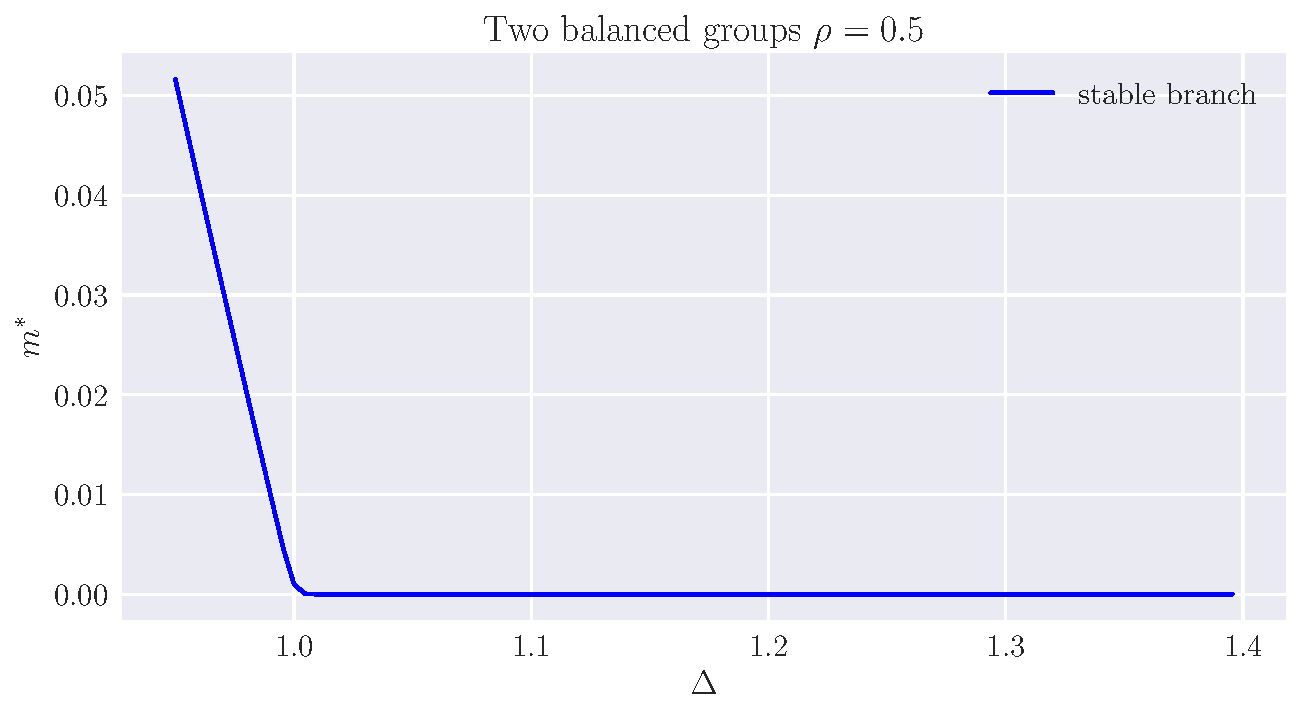
\includegraphics[width=400pt]{hw4/hw4_5_2.pdf}
            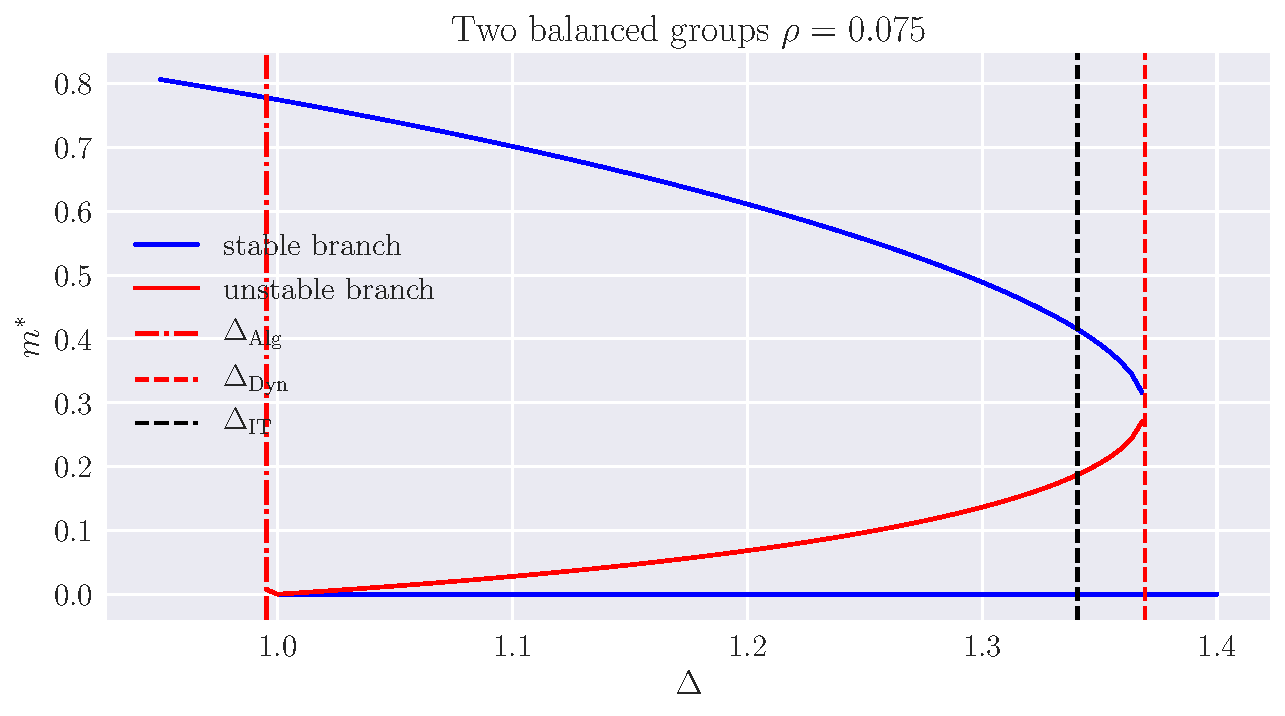
\includegraphics[width=400pt]{hw4/hw4_5_1.pdf}
        \end{figure}

\end{enumerate}
\end{solution}
        
\end{document}